% Official PSTA class downloaded 2026-10-24. Compile three times with pdflatex.
% The blind option suppresses identifying metadata in the review PDF.
\documentclass[blind]{psta}
\makeatletter
% Compatibility for the publisher's blind-mode placeholder; psta.cls is unchanged.
\providecommand{\HideFromPeer@}[1]{#1}
\makeatother
\usepackage{graphicx}
\usepackage{placeins}
\subjclass[UDC]{519.876.5}
\subjclass[2020]{93B30; 34A55, 65L09}
\JournalRubric{6}
\ArticleType{RAR}
\setlength{\emergencystretch}{2em}
\hfuzz=0.5pt
\hypersetup{pdfauthor={},pdfsubject={Finite-observation identification of a learning ODE},pdfkeywords={identifiability; learning dynamics; external assistance}}
\Russian

\title[Идентификация модели подготовки]{Идентификация динамической модели междисциплинарной подготовки при внешней поддержке}
% Identifying information is compiled out by the official blind option.
\author{Никитин, Пётр Владимирович}
\address{Финансовый университет при Правительстве Российской Федерации, Москва, Россия}
\email{pvnikitin@fa.ru}
\orcid{0000-0001-8866-5610}
\correspondent
\info{Кандидат педагогических наук, доцент кафедры искусственного интеллекта. Научные интересы: математическое моделирование образовательных процессов, программные системы поддержки обучения, междисциплинарная подготовка и применение искусственного интеллекта.}

\begin{abstract}
Рассматривается двухкомпонентная нелинейная модель междисциплинарной подготовки, учитывающая освоение, забывание, направленный перенос и внешнюю поддержку при выполнении заданий. Для девяти неизвестных параметров, включая начальные состояния и характеристики помощи, построен конечный протокол наблюдений. Для смешанного и полностью поддерживаемого режимов калибровки доказаны глобальная однозначность восстановления на образе модели, невырожденность якобиана отображения наблюдений и локальная устойчивость обратного отображения. Численный алгоритм сочетает явную калибровку, одномерное обращение и решение ограниченной задачи по двум параметрам освоения и переноса. Воспроизводимый эксперимент включает 80 синтетических восстановлений и 180000 повторений биномиальной калибровки. Исследовано ухудшение обусловленности при коротких интервалах наблюдения и почти постоянном состоянии предпосылки. Результаты задают требования к диагностическому протоколу и программному модулю идентификации. Девять точных вероятностей не отождествляются с девятью ответами одного обучающегося; применимость модели к реальным учебным событиям требует отдельной проверки.
\end{abstract}
\keywords{структурная идентифицируемость, динамическая модель, междисциплинарное обучение, внешняя поддержка, диагностика, численный эксперимент, интеллектуальная обучающая система}
\English
\title[Identifying a dynamic learning model]{Identifying a Dynamic Interdisciplinary Learning Model with External Assistance}
\author{Nikitin, Petr Vladimirovich}
\address{Financial University under the Government of the Russian Federation, Moscow, Russia}
\info{Candidate of Pedagogical Sciences, Associate Professor at the Department of Artificial Intelligence. Research interests include mathematical modelling of educational processes, learning support software, interdisciplinary learning, and artificial intelligence.}
\begin{abstract}
A two-component nonlinear model of interdisciplinary learning is considered, incorporating acquisition, forgetting, directed transfer, and external assistance in task completion. A finite observation protocol is constructed for nine unknown parameters, including initial states and assistance characteristics. For mixed and fully assisted calibration modes, global uniqueness of recovery on the model image, nonsingularity of the observation Jacobian, and local stability of the inverse map are established. The numerical algorithm combines explicit calibration, scalar inversion, and a constrained two-parameter acquisition-and-transfer fit. The reproducible experiment includes 80 synthetic recovery cases and 180000 binomial calibration replicates. The deterioration of conditioning with short observation intervals and an almost constant prerequisite state is examined. The results specify requirements for a diagnostic protocol and a software identification module. Nine exact probabilities do not represent nine responses from an individual learner; application to actual learning events requires separate validation.
\end{abstract}
\keywords{structural identifiability, dynamical model, interdisciplinary learning, external assistance, assessment, numerical experiment, intelligent learning system}
\begin{document}
\raggedbottom
\Russian
\maketitle
\pstamarkboth{Рукопись для рецензирования}{Идентификация модели подготовки}
\FloatBarrier
\section*{Введение}
Успешное выполнение задания с внешней поддержкой и способность самостоятельно решить сопоставимое задание характеризуют разные стороны подготовки. В модели индивидуальной траектории необходимо определить, при каких наблюдениях эти стороны можно разделить и какие учебные воздействия позволяют восстановить динамические параметры. В качестве первого предметного примера рассматриваются рекурсия и обход деревьев. Связь между ними трактуется как направленный перенос при практике по второму компоненту.

Различение скрытого состояния и наблюдаемого результата используется в моделях knowledge tracing \cite{ref1}. Современная классификация этих моделей приведена в обзоре \cite{ref2}, а проблемы интерпретируемости – в \cite{ref3}. Исследование смещения ответов \cite{ref4} показывает, что высокая точность прогноза сама по себе не подтверждает восстановление состояния знаний. Структурная идентифицируемость отвечает на вопрос об однозначности восстановления при точных наблюдениях \cite{ref5}. Её необходимо отличать от практической точности оценивания по конечным шумным данным \cite{ref6}. Современное обсуждение связи идентифицируемости, оценивания и прогнозирования дано в работе \cite{ref7}.

Протокол калибровки динамической модели должен согласовывать структуру, доступные наблюдения и процедуру оценивания \cite{ref8}. Средства анализа структурной идентифицируемости и наблюдаемости представлены, в частности, в STRIKE-GOLDD 4.0 \cite{ref9}. Анализ семейств моделей ОДУ \cite{ref10} показывает зависимость восстанавливаемых характеристик от наблюдаемых выходов. Эти работы используются как методологическая основа; биологические интерпретации их параметров на учебный процесс не переносятся.

Для линейных систем исследована идентификация по дискретным наблюдениям \cite{ref11}. Близкий препринт \cite{ref12} рассматривает обучение, забывание и перенос в системе ОДУ. Здесь изучается другая конкретная постановка: нелинейная связь через состояние компонента предпосылки, неизвестная поддержка в функции наблюдения и конечный протокол идентификации. Само использование ОДУ, насыщения или забывания не заявляется как научная новизна. Вклад работы состоит в конструктивном протоколе и доказательстве однозначности восстановления для заданной двухкомпонентной системы с неизвестной поддержкой.

В модели \cite{ref12} межкомпонентный перенос задаётся интенсивностями практики; при фиксированном входе уравнения состояний разделяются. В настоящей постановке скорость освоения второго компонента зависит от текущего состояния первого, поэтому сохраняется динамическая связь состояний. Структурная теорема в \cite{ref12} опирается на идеализацию наблюдаемой траектории состояния. Здесь рассматриваются конечные наблюдения вероятностей с неизвестными коэффициентами помощи. Таким образом, различаются и механизм переноса, и наблюдаемые величины; доказанный результат ограничен указанной моделью и протоколом.

Результат относится к условным вероятностям успеха для фиксированных калиброванных классов заданий. Одна бинарная отметка в журнале не является наблюдением такой вероятности. Девять вероятностей в теореме не означают девять ответов одного студента. Теоретическая идентифицируемость и оценивание этих вероятностей по данным рассматриваются раздельно.

Цель работы – установить условия, при которых конечные наблюдения разделяют изменение самостоятельной подготовки, перенос между компонентами и влияние внешней помощи. Сначала задаются модель и протокол, затем обосновываются восстановление и его устойчивость. После описания вычислительного алгоритма приводятся синтетическая проверка и границы применения результата.

\FloatBarrier
\section{Модель подготовки и механизм наблюдений}
Пусть $x_{1}$ и $x_{2}$ – состояния самостоятельной подготовки по двум компонентам, нормированные на интервал от нуля до единицы; $u_{1}$ и $u_{2}$ – известные неотрицательные интенсивности практики. Время измеряется в условных учебных периодах. Рассматривается система (1), (2)

\begin{equation}
\dot x_1=\alpha_1u_1(t)(1-x_1)-\lambda_1x_1,\qquad x_1(0)=X_1,
\tag{1}
\label{eq:1}
\end{equation}
\begin{equation}
\dot x_2=u_2(t)(\alpha_2+\beta x_1)(1-x_2)-\lambda_2x_2,\qquad x_2(0)=X_2.
\tag{2}
\label{eq:2}
\end{equation}
Коэффициенты $\alpha_{1}$ и $\alpha_{2}$ характеризуют освоение при практике, $\lambda_{1}$ и $\lambda_{2}$ – забывание, $\beta$ – усиление освоения второго компонента при наличии первой предпосылки. Перенос действует только при $u_{2}$ > 0. Таким образом, модель не предполагает самопроизвольного освоения второго компонента без практики. Вероятность наблюдаемого успеха задаётся формулой (3).

\begin{equation}
p_i(t,\chi )=\chi \eta_i+(1-\chi \eta_i)x_i(t),\qquad \chi \in\{0,1\},\quad i=1,2.
\tag{3}
\label{eq:3}
\end{equation}
Здесь $\chi$ = 0 обозначает самостоятельную диагностику, $\chi$ = 1 – диагностику с поддержкой. Параметр $\eta_{i}$ – условная вероятность успешной поддержки, когда самостоятельного выполнения недостаточно. Это допущение о механизме наблюдения, а не универсальное свойство генеративного ИИ. Влияние помощи на последующее обучение в данной версии отдельно не параметризовано. Диагностические измерения считаются мгновенными и не изменяют состояние.

\[
\psi=(X_1,\lambda_1,\eta_1,X_2,\lambda_2,\eta_2,\alpha_1,\alpha_2,\beta)\in\Theta,
\]
\[
\begin{aligned}\Theta=&(0,1)\times(0,\infty)\times(0,1)\\&\times(0,1)\times(0,\infty)\times(0,1)\\&\times(0,\infty)^3.\end{aligned}
\]
Шкала состояния и классы заданий фиксированы. Неизвестные трудности, угадывание, ошибки оценщика, разная интенсивность поддержки и различающиеся между студентами параметры требуют расширения модели и не входят в доказанную ниже теорему. В частности, $x_{i}$ не отождествляется с полнотой сформированности всей компетенции выпускника.

\par\medskip\noindent\textbf{Лемма 1. Для любого $\psi$ из $\Theta$ и ограниченных кусочно постоянных неотрицательных управлений решение существует единственно при всех t $\ge$ 0 и принадлежит открытому квадрату (0,1)$^{2}$ на каждом конечном интервале.}\par\smallskip
Доказательство. Правая часть локально липшицева по состоянию на каждом участке постоянного управления. Неравенство $\dot{x}_{1}$ $\ge$ $-$$\lambda_{1}$$x_{1}$ сохраняет положительность $x_{1}$. Для $z_{1}$ = 1 $-$ $x_{1}$ имеем $\dot{z}_{1}$ = $\lambda_{1}$ $-$ ($\alpha_{1}$$u_{1}$ + $\lambda_{1}$)$z_{1}$, что сохраняет $z_{1}$ > 0. После установления 0 < $x_{1}$ < 1 аналогичные оценки применяются ко второму уравнению и $z_{2}$ = 1 $-$ $x_{2}$. Ограниченность состояния исключает конечный уход решения на бесконечность. На границах участков решения склеиваются непрерывно и единственно. Лемма доказана.

\FloatBarrier
\section{Протокол и конструктивное восстановление параметров}
Фиксируются h > 0, L > 0, $c_{1}$ > 0, $c_{2}$ > 0 и 0 < $t_{1}$ < $t_{2}$. Обозначим $T_{0}$ = 2h и $T_{1}$ = 2h + L. В таблице 1 приведён протокол; у каждого компонента на калибровочном участке выбирается один и тот же вариант M или A.

\begin{table}[htbp]
\caption{Протокол идентификации}
\label{tab:22}
\centering\small
\renewcommand{\arraystretch}{1.25}
\setlength{\tabcolsep}{3pt}
\begin{tabular}{|p{.20\linewidth}|p{.22\linewidth}|p{.47\linewidth}|}
\hline
\textbf{Участок} & \textbf{Управление} & \textbf{Наблюдения}\\\hline
0 $\le$ t $\le$ 2h & $u_{1}$ = $u_{2}$ = 0 & По три вероятности для каждого компонента в 0, h, 2h\\\hline
2h < t $\le$ $T_{1}$ & $u_{1}$ = $c_{1}$, $u_{2}$ = 0 & Вероятность первого компонента при t = $T_{1}$\\\hline
$T_{1}$ < t $\le$ $T_{1}$ + $t_{2}$ & $u_{1}$ = 0, $u_{2}$ = $c_{2}$ & Вероятности второго компонента при $T_{1}$ + $t_{1}$ и $T_{1}$ + $t_{2}$\\\hline
\end{tabular}
\end{table}
Вариант M использует режимы (0,0,1) в моменты (0,h,2h), вариант A – режимы (1,1,1). Все три последующих измерения выполняются с поддержкой. После калибровки $\eta_{i}$ они однозначно пересчитываются в состояния по формуле $x_{i}$ = ($p_{i}$ $-$ $\eta_{i}$)/(1 $-$ $\eta_{i}$). Итого наблюдаются девять скалярных вероятностей. Конечные мгновенные измерения при переключении не меняют непрерывную траекторию.

Участок без практики является условием математического протокола. В реальном курсе отсутствие дополнительного обучения по тем же компонентам необходимо проверять, а диагностическая активность сама может нарушать это условие. Поэтому протокол пока используется как исследовательская конструкция для синтетической проверки.

Рассмотрим один компонент и обозначим X = x(0), $\lambda$ = $\lambda_{i}$, $\eta$ = $\eta_{i}$ и $\kappa$ = exp($-$$\lambda$h). На первом участке x(kh) = X$\kappa$$^{k}$. Пусть $P_{0}$, $P_{1}$, $P_{2}$ – три соответствующие вероятности.

\par\medskip\noindent\textbf{Предложение 1. Вариант M глобально определяет X, $\lambda$ и $\eta$ на заданной области параметров по формулам}\par\smallskip
\[
X=P_0,\qquad \kappa =P_1/P_0,\qquad \lambda=-h^{-1}\ln \kappa ,
\]
\[
\eta=\frac{P_2-X\kappa ^2}{1-X\kappa ^2}.
\]
\par\medskip\noindent\textbf{Вариант A также глобально определяет эти параметры по формулам}\par\smallskip
\[
\kappa =\frac{P_1-P_2}{P_0-P_1},\qquad \lambda=-h^{-1}\ln \kappa ,
\]
\[
\eta=\frac{P_1-\kappa P_0}{1-\kappa },\qquad X=\frac{P_0-\eta}{1-\eta}.
\]
Доказательство. В варианте M имеем $P_{0}$ = X, $P_{1}$ = X$\kappa$ и $P_{2}$ = $\eta$ + (1 $-$ $\eta$)X$\kappa$$^{2}$. Знаменатель 1 $-$ X$\kappa$$^{2}$ положителен. В варианте A $P_{k}$ = $\eta$ + (1 $-$ $\eta$)X$\kappa$$^{k}$; последовательные разности равны (1 $-$ $\eta$)X(1 $-$ $\kappa$) и (1 $-$ $\eta$)X$\kappa$(1 $-$ $\kappa$). Так как 0 < $\kappa$ < 1, обе разности и все используемые знаменатели положительны. Их отношение даёт $\kappa$, после чего $\eta$ и X восстанавливаются однозначно. Предложение доказано.

\par\medskip\noindent\textbf{Предложение 2. Определители якобианов калибровочных отображений по переменным (X,$\lambda$,$\eta$) равны}\par\smallskip
\begin{equation}
\det J_M=-hX\kappa (1-X\kappa ^2),\qquad \det J_A=-hX(1-\eta)^2\kappa (1-\kappa )^2.
\tag{4}
\label{eq:4}
\end{equation}
Доказательство. Для k = 0,1,2 строка соответствующего якобиана имеет вид ((1 $-$ $\chi_{k}$$\eta$)$\kappa$$^{k}$, $-$(1 $-$ $\chi_{k}$$\eta$)hkX$\kappa$$^{k}$, $\chi_{k}$(1 $-$ X$\kappa$$^{k}$)). Подстановка $\chi$ = (0,0,1) и $\chi$ = (1,1,1) и вычисление определителей дают указанные выражения. Ни один определитель не равен нулю в $\Theta$. Предложение доказано.

Определители (4) дают следующее сравнение. При фиксированных внутренних значениях X, $\lambda$ и $\eta$ и h $\to$ 0 получаем det $J_{M}$ = $-$X(1 $-$ X)h + O(h$^{2}$), det $J_{A}$ = $-$X(1 $-$ $\eta$)$^{2}$$\lambda$$^{2}$h$^{3}$ + O(h$^{4}$). Это сравнение объёмного сжатия отображений не заменяет анализа наименьшего сингулярного числа. Оно показывает дополнительное вырождение полностью поддерживаемой калибровки при коротком интервале; универсального превосходства M для любых шумов и расписаний из него не следует.

В полностью поддерживаемом режиме восстановление постоянного слагаемого и одной экспоненты является частным случаем классической задачи оценивания экспоненциальных сумм \cite{ref13}. Эти алгебраические формулы не предлагаются как новый вариант метода Прони. Их роль здесь – калибровка неизвестной поддержки перед идентификацией нелинейного междисциплинарного взаимодействия.

После калибровки известны шесть параметров и состояния в конце первого участка. Из измерения первого компонента в $T_{1}$ получаем A = $x_{1}$($T_{1}$). На втором участке коэффициент $\alpha_{1}$ восстанавливается из скалярного уравнения

\[
\begin{aligned}A=&\frac{\alpha_1c_1}{k}\\&+\left(X_1e^{-2h\lambda_1}-\frac{\alpha_1c_1}{k}\right)e^{-kL},\\k=&\alpha_1c_1+\lambda_1.\end{aligned}
\]
Производная конечного состояния по $\alpha_{1}$ положительна: соответствующая чувствительность удовлетворяет линейному уравнению с нулевым начальным условием и строго положительным источником $c_{1}$(1 $-$ $x_{1}$). Следовательно, конечное состояние строго возрастает по $\alpha_{1}$ и указанное уравнение имеет не более одного решения. Для наблюдений, порождённых моделью, решение существует.

Перенесём начало времени в $T_{1}$ и обозначим B = $x_{2}$($T_{1}$). Тогда на последнем участке

\[
w(t)=Ae^{-\lambda_1t},\qquad B=X_2e^{-\lambda_2(2h+L)},
\]
\[
\dot z=c_2(\alpha+\beta w(t))(1-z)-\lambda_2z,\qquad z(0)=B,\quad \alpha=\alpha_2.
\]
\par\medskip\noindent\textbf{Лемма 2. Если A > 0, $\lambda_{1}$ > 0, 0 < B < 1, $c_{2}$ > 0 и 0 < $t_{1}$ < $t_{2}$, то отображение ($\alpha$,$\beta$) $\mapsto$ (z($t_{1}$),z($t_{2}$)) глобально инъективно на положительном квадранте. Его якобиан невырожден в каждой точке этого квадранта.}\par\smallskip
Доказательство глобальной однозначности. Пусть две пары параметров дают одинаковые значения z в $t_{1}$ и $t_{2}$. Обозначим разность решений v = z $-$ $\widetilde{z}$, $\delta$$\alpha$ = $\alpha$ $-$ $\widetilde{\alpha}$ и $\delta$$\beta$ = $\beta$ $-$ $\widetilde{\beta}$. Тогда

\[
\dot v+k(t)v=c_2(\delta\alpha+\delta\beta w(t))(1-\widetilde z(t)),\quad v(0)=0,
\]
\[
k(t)=c_2(\alpha+\beta w(t))+\lambda_2.
\]
После умножения на положительный интегрирующий множитель условие v($t_{1}$) = 0 даёт нулевой интеграл функции g(t) = $\delta$$\alpha$ + $\delta$$\beta$w(t) с положительным весом на (0,$t_{1}$). Из v($t_{2}$) = v($t_{1}$) = 0 следует такой же нулевой интеграл на ($t_{1}$,$t_{2}$). При $\delta$$\beta$ $\ne$ 0 функция g строго монотонна и имеет не более одного нуля. Первый нулевой интеграл требует смены знака внутри (0,$t_{1}$), после чего на ($t_{1}$,$t_{2}$) знак постоянен и второй интеграл не может быть нулевым. Если $\delta$$\beta$ = 0, первый интеграл требует $\delta$$\alpha$ = 0. Следовательно, обе пары совпадают.

Доказательство невырожденности. Положим K(t) = $\int_0^t$k(s)ds и W(s) = exp(K(s))(1 $-$ z(s)) > 0. Чувствительности по $\alpha$ и $\beta$ равны

\[
\begin{aligned}S_\alpha(t)&=c_2e^{-K(t)}\int_0^tW(s)\,ds,\\S_\beta(t)&=c_2e^{-K(t)}\int_0^tW(s)w(s)\,ds.\end{aligned}
\]
Отношение R(t) = S$\beta$(t)/S$\alpha$(t) является средним строго убывающей функции w с положительным весом на (0,t). Поэтому R(t) > w(t) и

\[
R^{\prime}(t)=\frac{W(t)}{\int_0^t W(s)\,ds}\bigl(w(t)-R(t)\bigr)<0.
\]
\[
\det J_{\alpha,\beta}=S_\alpha(t_1)S_\alpha(t_2)\bigl(R(t_2)-R(t_1)\bigr)<0.
\]
Лемма доказана. Существенна изменяемость состояния предпосылки w во времени. Два измерения одной и той же постоянной комбинации $\alpha$ + $\beta$w не разделяют $\alpha$ и $\beta$.

\FloatBarrier
\section{Идентифицируемость и устойчивость восстановления}
\par\medskip\noindent\textbf{Теорема 1. Пусть $\psi$ принадлежит $\Theta$, выполнены условия описанного протокола и наблюдаются девять точных вероятностей. Для каждого из вариантов M и A полный вектор $\psi$ восстанавливается глобально однозначно. Отображение F из $\Theta$ в $\mathbb{R}$$^{9}$, сопоставляющее параметрам эти вероятности, имеет невырожденный якобиан во всех точках $\Theta$.}\par\smallskip
Доказательство. По предложению 1 первые шесть наблюдений восстанавливают ($X_{1}$,$\lambda_{1}$,$\eta_{1}$,$X_{2}$,$\lambda_{2}$,$\eta_{2}$). Седьмое наблюдение определяет A, а затем единственное $\alpha_{1}$ по строгой монотонности конечного состояния на втором участке. Состояние B известно из калибровки. Последние два наблюдения определяют z($t_{1}$), z($t_{2}$), а лемма 2 единственным образом определяет $\alpha_{2}$ и $\beta$. Это доказывает глобальную однозначность.

При указанном порядке параметров якобиан является блочно нижнетреугольным. Два верхних диагональных блока – калибровочные якобианы. Оставшийся блок содержит в первой строке только ненулевую производную седьмого наблюдения по $\alpha_{1}$, а в нижнем правом углу – (1 $-$ $\eta_{2}$)$J_{\alpha,\beta}$. Поэтому определитель полного отображения имеет вид (5).

\begin{equation}
\begin{aligned}\det DF=&\det J_1\det J_2(1-\eta_1)\frac{\partial A}{\partial\alpha_1}\\&\times(1-\eta_2)^2\det J_{\alpha,\beta}\ne0.\end{aligned}
\tag{5}
\label{eq:5}
\end{equation}
Гладкость отображения следует из гладкой зависимости решений от параметров при фиксированном протоколе. Все множители в последней формуле ненулевые. Теорема доказана.

Теорема устанавливает однозначность на образе F($\Theta$). Она не утверждает, что произвольный набор девяти эмпирических частот соответствует допустимому $\psi$. Число девять совпадает с размерностью параметризации; при меньшем числе скалярных наблюдений дифференцируемое обратное отображение полного вектора невозможно по рангу якобиана. Это замечание относится к регулярному локальному восстановлению, а не к универсальной оптимальности диагностического дизайна.

\par\medskip\noindent\textbf{Теорема 2. Для любой внутренней точки $\psi_{0}$ существует выпуклая окрестность U, в которой для любых $\psi$ и $\widetilde{\psi}$ выполнено неравенство}\par\smallskip
\begin{equation}
\begin{aligned}\|\psi-\widetilde\psi\|_2&\le\frac{2}{\sigma_0}\|F(\psi)-F(\widetilde\psi)\|_2,\\\sigma_0&=\sigma_{\min}(DF(\psi_0))>0.\end{aligned}
\tag{6}
\label{eq:6}
\end{equation}
Доказательство. По непрерывности DF выбирается выпуклая окрестность, в которой $\Vert$DF($\psi$) $-$ DF($\psi_{0}$)$\Vert$$_{2}$ $\le$ $\sigma_{0}$/2. Интегральная формула приращения даёт F($\psi$) $-$ F($\widetilde{\psi}$) = DF($\psi_{0}$)($\psi$ $-$ $\widetilde{\psi}$) + E, где $\Vert$E$\Vert$$_{2}$ $\le$ ($\sigma_{0}$/2)$\Vert$$\psi$ $-$ $\widetilde{\psi}$$\Vert$$_{2}$. Из определения наименьшего сингулярного числа получаем нижнюю оценку $\Vert$F($\psi$) $-$ F($\widetilde{\psi}$)$\Vert$$_{2}$ $\ge$ ($\sigma_{0}$/2)$\Vert$$\psi$ $-$ $\widetilde{\psi}$$\Vert$$_{2}$. Теорема доказана.

Из оценки (6) следует, что если оценка $\widehat{\psi}$ принадлежит U, ошибка вероятностей не превосходит $\varepsilon$, а невязка $\Vert$F($\widehat{\psi}$) $-$ $\widehat{p}$$\Vert$$_{2}$ не превосходит $\omega$, то

\[
\|\widehat\psi-\psi_0\|_2\le\frac{2}{\sigma_0}(\varepsilon+\omega).
\]
Условие $\widehat{\psi}$ $\in$ U существенно. Полученная оценка не гарантирует сходимости оптимизатора из произвольной начальной точки и не является глобальной равномерной оценкой вблизи вырожденных режимов.

Для связи с бинарными ответами рассмотрим статистическую идеализацию: в каждой из девяти ячеек выполнено n независимых бернуллиевских испытаний с одной и той же фиксированной вероятностью. По неравенству Хёффдинга \cite{ref14} и объединению девяти событий с вероятностью не меньше 1 $-$ $\zeta$ имеем

\[
\begin{aligned}\|\widehat p-p\|_\infty&\le\sqrt{\frac{\ln(18/\zeta)}{2n}},\\\|\widehat p-p\|_2&\le3\sqrt{\frac{\ln(18/\zeta)}{2n}}.\end{aligned}
\]
Испытания внутри ячейки должны иметь одинаковое состояние и сопоставимую трудность. Последовательные учебные задания обычно изменяют состояние, поэтому механическое повторение задания одному студенту не реализует эту идеализацию. Для реальных данных потребуется вероятностная модель по отдельным событиям и дополнительная проверка наблюдательного механизма.

Если на последнем участке w(t) = $w_{0}$ постоянно, уравнение второго компонента зависит от $\alpha_{2}$ и $\beta$ только через $\alpha_{2}$ + $\beta$$w_{0}$. Для любого достаточно малого d пары ($\alpha_{2}$,$\beta$) и ($\alpha_{2}$ $-$ $w_{0}$d,$\beta$ + d) порождают одну и ту же траекторию. Например, при $w_{0}$ = 0,6 пары (0,4; 0,9) и (0,25; 1,15) дают одинаковое значение 0,94. Все параметры в этом примере положительны. Следовательно, две точные диагностики сами по себе не обеспечивают разделения освоения и переноса.

Аналогичная проблема возникает при стационарных наблюдениях и постоянном управлении. Равновесие первого компонента определяет только отношение $\alpha_{1}$$u_{1}$/$\lambda_{1}$. Одновременное умножение $\alpha_{1}$ и $\lambda_{1}$ на положительную константу не меняет этого равновесия. Даже наличие самостоятельных измерений не устраняет отсутствие динамического возбуждения.

Вариант A теряет калибровочную идентифицируемость при $\lambda$ = 0: все три вероятности совпадают и параметры X и $\eta$ смешиваются. Эти граничные случаи не входят в $\Theta$, но близость к ним ухудшает численную устойчивость. Данные с поддержкой нельзя объявлять ни всегда неинформативными, ни всегда достаточными.

\FloatBarrier
\section{Вычислительный алгоритм и исследовательская реализация}
Исследовательская программа реализует последовательную идентификацию, следующую из теоремы 1. На вход подаются девять вероятностей и известное расписание учебных воздействий. Для данных в допустимом образе сначала вычисляются параметры калибровки двух компонентов. Затем из седьмого наблюдения определяется состояние предпосылки и решается скалярное уравнение для $\alpha_{1}$. На последнем шаге два оставшихся параметра определяются по двум наблюдениям второго компонента.

Скалярное уравнение решается методом Брента после проверки знаков на концах интервала. Для пары ($\alpha_{2}$,$\beta$) применяется ограниченный метод наименьших квадратов с аналитическим якобианом чувствительностей. Используются стандартные средства SciPy \cite{ref15}. Если прямые формулы калибровки выходят за область параметров, программа фиксирует отказ такого обращения и сохраняет исходные частоты. Автоматическое обрезание параметров до допустимых границ изменило бы обратную задачу и не используется в данном эксперименте.

Прямая задача на последнем участке решается по формуле вариации постоянных. В обозначениях леммы 2 вводятся K(t) = $\int_0^t$[$c_{2}$($\alpha_{2}$ + $\beta$w(s)) + $\lambda_{2}$]ds и z(0) = B. Тогда 1 $-$ z(t) = (1 $-$ B)exp($-$K(t)) + $\lambda_{2}$$\int_0^t$exp(K(s) $-$ K(t))ds. Запись через разность K(s) $-$ K(t) позволяет избежать положительных больших экспонент. Интеграл вычисляется квадратурой с 64 узлами. Независимый контроль использует интегрирование исходной системы, а не ту же интегральную формулу.

При фиксированном числе узлов стоимость прямого расчёта и аналитических чувствительностей пропорциональна числу запрошенных моментов. Стоимость обратного расчёта дополнительно зависит от числа итераций методов поиска корня и наименьших квадратов. Глобальная сходимость оптимизатора из произвольной начальной точки из теоремы об идентифицируемости не следует. Поэтому сохраняются начальная точка, ограничения, невязка и признак завершения расчёта.

Реализован вычислительный исследовательский модуль. Его связь с учебным журналом задаётся через записи о компоненте, классе задания, времени, учебном воздействии и режиме поддержки. Подключение модуля к рабочему образовательному комплексу и проверка на реальных событиях рассматриваются как следующий этап. Входные вероятности нельзя непосредственно заменить оценкой за одно задание или усреднить между разными студентами без модели неоднородности.

\FloatBarrier
\section{Вычислительный эксперимент}
Программа experiment.py использует генератор NumPy с seed = 20261022. Для 40 случайных допустимых векторов параметров проверены оба протокола, всего 80 случаев восстановления. Прямая задача на последнем участке вычисляется по формуле вариации постоянных с 64 узлами квадратуры Гаусса – Лежандра. Независимый контроль выполнен интегратором DOP853 для исходной системы ОДУ. Коэффициент $\alpha_{1}$ определяется скалярным методом Брента, $\alpha_{2}$ и $\beta$ – методом ограниченных наименьших квадратов с аналитическими чувствительностями. Общая сходимость этих вычислительных процедур в статье не доказывается.

Максимальная абсолютная ошибка восстановления параметров в 80 случаях составила 4,647$\cdot$10$^{-13}$, а максимальное расхождение прямого расчёта с независимым интегрированием – 7,403$\cdot$10$^{-13}$. Эти величины описывают проверенный диапазон синтетических конфигураций и не заменяют доказательства теоремы. Две формулы калибровочных определителей дополнительно проверены символьными вычислениями.

Для исследования обусловленности фиксированы $X_{1}$ = 0,65, $\lambda_{1}$ = 0,22, $\eta_{1}$ = 0,45, $X_{2}$ = 0,50, $\lambda_{2}$ = 0,15, $\eta_{2}$ = 0,35, $\alpha_{1}$ = 0,70, $\alpha_{2}$ = 0,40, $\beta$ = 0,90. Остальные параметры протокола: L = 2, $c_{1}$ = $c_{2}$ = 1, $t_{1}$ = 1,5, $t_{2}$ = 4. Сингулярные числа относятся к указанным единицам измерения и данной параметризации.

\begin{table}[htbp]
\caption{Наименьшие сингулярные числа}
\label{tab:84}
\centering\small
\renewcommand{\arraystretch}{1.25}
\setlength{\tabcolsep}{3pt}
\begin{tabular}{|c|c|p{.24\linewidth}|p{.30\linewidth}|}
\hline
\textbf{h} & \textbf{Режим} & \textbf{Калибровка $\sigma_{\min}$} & \textbf{Полное DF $\sigma_{\min}$}\\\hline
0,1 & M & 4,501$\cdot$10$^{-2}$ & 3,157$\cdot$10$^{-3}$\\\hline
0,1 & A & 1,472$\cdot$10$^{-4}$ & 2,615$\cdot$10$^{-5}$\\\hline
1 & M & 3,169$\cdot$10$^{-1}$ & 1,681$\cdot$10$^{-2}$\\\hline
1 & A & 1,391$\cdot$10$^{-2}$ & 1,952$\cdot$10$^{-3}$\\\hline
4 & M & 7,156$\cdot$10$^{-1}$ & 2,095$\cdot$10$^{-2}$\\\hline
4 & A & 1,494$\cdot$10$^{-1}$ & 1,203$\cdot$10$^{-2}$\\\hline
\end{tabular}
\end{table}
На рисунке 1 приведены две зависимости: уменьшение информативности короткой калибровки и вырождение разделения освоения и переноса при почти постоянной предпосылке. Нормировка параметров фиксирована и совпадает с нормировкой таблицы 2.

\begin{figure}[htbp]
\centering
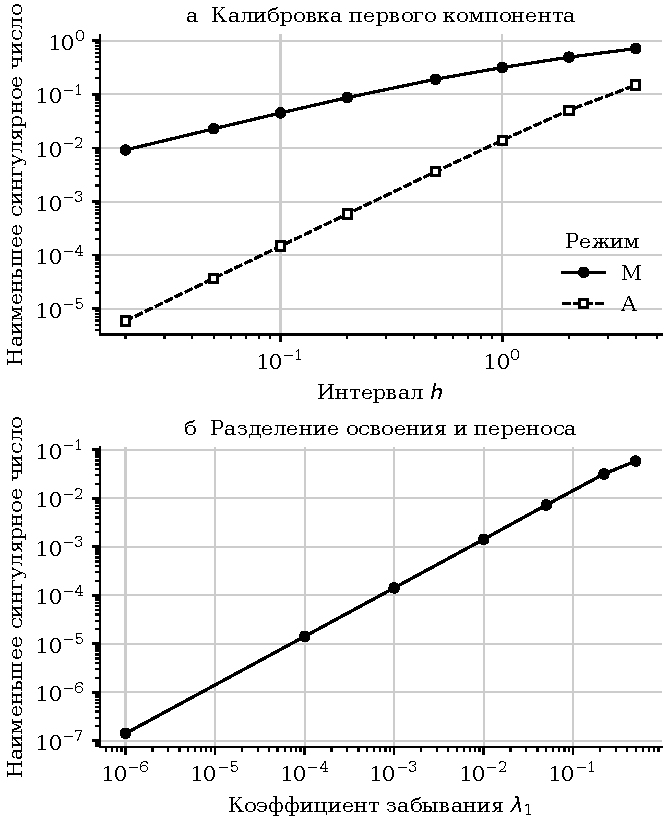
\includegraphics[width=.98\linewidth]{figures/conditioning.pdf}
\caption{Обусловленность калибровки и идентификации переноса}
\label{fig:conditioning}
\end{figure}
Отдельно выполнены 18 конфигураций биномиального моделирования калибровки первого компонента: h $\in$ \{0,1; 1; 3\}, n $\in$ \{1000; 10000; 100000\}, режимы M и A. На конфигурацию использованы 10000 повторений, всего 180000 синтетических троек частот. Фиксируются доля троек вне допустимого образа замкнутых формул и ошибка $\eta$ среди допустимых троек. Такая доля характеризует прямое обращение формул, а не невозможность подбора ограниченной модели методом максимального правдоподобия.

\begin{table}[htbp]
\caption{Калибровка при n равном 10000}
\label{tab:88}
\centering\small
\renewcommand{\arraystretch}{1.25}
\setlength{\tabcolsep}{3pt}
\begin{tabular}{|c|c|p{.24\linewidth}|p{.30\linewidth}|}
\hline
\textbf{h} & \textbf{Режим} & \textbf{Вне образа \%} & \textbf{Медиана ошибки $\eta$ условная}\\\hline
0,1 & M & 1,88 & 0,0120\\\hline
0,1 & A & 57,98 & 0,3368\\\hline
1,0 & M & 0,00 & 0,0079\\\hline
1,0 & A & 21,89 & 0,1039\\\hline
3,0 & M & 0,00 & 0,0046\\\hline
3,0 & A & 0,00 & 0,0210\\\hline
\end{tabular}
\end{table}
Условную медиану следует читать вместе с долей недопустимых троек: исключение таких троек не является успешным оцениванием. Полные результаты, включая 90-й процентиль ошибок, находятся в CSV и JSON воспроизводимого пакета. Отдельный расчёт при $\lambda_{1}$ $\to$ 0 показывает уменьшение наименьшего сингулярного числа блока переноса, согласованное с контрпримером постоянной предпосылки.

Таблица 2 сопоставляет обусловленность калибровки и полного отображения наблюдений; таблица 3 – чувствительность прямых формул к биномиальному шуму. При h = 0,1 и n = 10000 доля троек вне допустимого образа составила 1,88 \% для M и 57,98 \% для A. При h = 3 в этой конфигурации обе доли равны нулю. Эти результаты не устанавливают оптимальное расписание для всех параметров или моделей ошибок.

\FloatBarrier
\section{Применение и ограничения}
Для пары «рекурсия – обход деревьев» $x_{1}$ и $x_{2}$ можно связать с вероятностями самостоятельного выполнения заранее калиброванных семейств задач. $\beta$ описывает изменение темпа освоения обходов при более высоком состоянии рекурсивной подготовки. Наличие такой связи не устанавливает причинный эффект обучения без контроля альтернативных объяснений и внешних учебных воздействий.

В междисциплинарном варианте возможна пара «комбинаторные структуры» из дискретной математики и «графовые алгоритмы». Та же математическая конструкция переносится на новую пару только после проверки наблюдательной модели и содержательной интерпретации параметров. Доказательство для двух компонентов не распространяется автоматически на произвольный граф всех дисциплин четырёхлетней программы.

Для программного комплекса результат задаёт требования к данным: идентификатор компонента и семейства задания, момент наблюдения, режим поддержки, известное учебное воздействие и версия параметризации. При оценивании необходимо хранить невязку, чувствительности и диагностические признаки плохой обусловленности. Изменения базы данных и интерфейса в рамках данной математической работы не выполнялись.

\FloatBarrier
\section*{Заключение}
Для двухкомпонентной модели междисциплинарной подготовки построен конечный протокол восстановления девяти неизвестных параметров, включая характеристики внешней поддержки. Доказаны глобальная однозначность восстановления на образе модели, невырожденность якобиана и локальная устойчивость обратного отображения. Контрпример постоянной предпосылки указывает на необходимость динамически информативного расписания.

Исследовательская реализация проверена на 80 синтетических случаях восстановления и 180000 статистических повторениях калибровки. Сравнение режимов M и A показывает роль независимых диагностических наблюдений при коротком интервале. Следующие задачи – проверка наблюдательного механизма по индивидуальным учебным событиям и расширение идентификационного протокола на несколько взаимосвязанных компонентов.

\FloatBarrier
\begin{thebibliography}{99}
\Bibitem{ref1}
\by Corbett A.T., Anderson J.R.
\paper Knowledge tracing: Modeling the acquisition of procedural knowledge
\jour User Modeling and User-Adapted Interaction
\yr 1994
\vol 4
\pages 253--278
\doi 10.1007/BF01099821

\Bibitem{ref2}
\by Abdelrahman G., Wang Q., Nunes B.
\paper Knowledge tracing: A survey
\jour ACM Computing Surveys
\yr 2023
\vol 55
\issue 11
\miscnote Art. 224. P. 1–37
\doi 10.1145/3569576

\Bibitem{ref3}
\by Bai Y., Zhao J., Wei T., Cai Q., He L.
\paper A survey of explainable knowledge tracing
\jour Applied Intelligence
\yr 2024
\vol 54
\issue 8
\pages 6483--6514
\doi 10.1007/s10489-024-05509-8

\Bibitem{ref4}
\by Cui C., Ma H., Dong X., Zhang C., Zhang C., Yao Y., Chen M., Ma Y.
\paper Model-agnostic counterfactual reasoning for identifying and mitigating answer bias in knowledge tracing
\jour Neural Networks
\yr 2024
\vol 178
\miscnote Art. 106495
\doi 10.1016/j.neunet.2024.106495

\Bibitem{ref5}
\by Bellman R., Åström K.J.
\paper On structural identifiability
\jour Mathematical Biosciences
\yr 1970
\vol 7
\issue 3–4
\pages 329--339
\doi 10.1016/0025-5564(70)90132-X

\Bibitem{ref6}
\by Miao H., Xia X., Perelson A.S., Wu H.
\paper On identifiability of nonlinear ODE models and applications in viral dynamics
\jour SIAM Review
\yr 2011
\vol 53
\issue 1
\pages 3--39
\doi 10.1137/090757009

\Bibitem{ref7}
\by Simpson M.J., Baker R.E.
\paper Parameter identifiability, parameter estimation, and model prediction for differential equation models
\jour SIAM Review
\yr 2026
\vol 68
\issue 1
\pages 153--171
\doi 10.1137/24M1667968

\Bibitem{ref8}
\by Villaverde A.F., Pathirana D., Fröhlich F., Hasenauer J., Banga J.R.
\paper A protocol for dynamic model calibration
\jour Briefings in Bioinformatics
\yr 2022
\vol 23
\issue 1
\miscnote Art. bbab387
\doi 10.1093/bib/bbab387

\Bibitem{ref9}
\by Díaz-Seoane S., Rey Barreiro X., Villaverde A.F.
\paper STRIKE-GOLDD 4.0: user-friendly, efficient analysis of structural identifiability and observability
\jour Bioinformatics
\yr 2023
\vol 39
\issue 1
\miscnote Art. btac748
\doi 10.1093/bioinformatics/btac748

\Bibitem{ref10}
\by Massonis G., Banga J.R., Villaverde A.F.
\paper Structural identifiability and observability of compartmental models of the COVID-19 pandemic
\jour Annual Reviews in Control
\yr 2021
\vol 51
\pages 441--459
\doi 10.1016/j.arcontrol.2020.12.001

\Bibitem{ref11}
\by Wang Y., Huang W., Gong M., Geng X., Liu T., Zhang K., Tao D.
\paper Identifiability and asymptotics in learning homogeneous linear ODE systems from discrete observations
\jour Journal of Machine Learning Research
\yr 2024
\vol 25
\issue 154
\pages 1--50
\url https://jmlr.org/papers/v25/22-1159.html

\Bibitem{ref12}
\by Kostanian A., Beklaryan A.
\paper Identifiability of a dissipative knowledge-dynamics model: exact recovery under designed excitation, degeneration on observational data
\miscnote Preprint, version 3, 15 October 2026
\yr 2026
\arxiv 2610.09889v3
\doi 10.48550/arXiv.2610.09889

\Bibitem{ref13}
\by Potts D., Tasche M.
\paper Parameter estimation for exponential sums by approximate Prony method
\jour Signal Processing
\yr 2010
\vol 90
\issue 5
\pages 1631--1642
\doi 10.1016/j.sigpro.2009.11.012

\Bibitem{ref14}
\by Hoeffding W.
\paper Probability inequalities for sums of bounded random variables
\jour Journal of the American Statistical Association
\yr 1963
\vol 58
\issue 301
\pages 13--30
\doi 10.1080/01621459.1963.10500830

\Bibitem{ref15}
\by Virtanen P., Gommers R., Oliphant T.E. et al.
\paper SciPy 1.0: fundamental algorithms for scientific computing in Python
\jour Nature Methods
\yr 2020
\vol 17
\issue 3
\pages 261--272
\doi 10.1038/s41592-019-0686-2

\end{thebibliography}
\makefinish
\English
\maketitle
\end{document}
